% Welcome! This is the unofficial University of Udine beamer template.

% We defined four theme colors: UniBrown, UniBlue, UniGold
% and UniOrange. For example, to write some uniud-brownish
% text, just use: \textcolor{UniBrown}{Hello!}

\documentclass[usenames,dvipsnames]{beamer}
\usepackage[utf8]{inputenc}
\usepackage{verbatim}
\usetheme{uniud}
%\bibliography{bib}
%%% Bibliography
%\usepackage[style=authoryear,backend=biber]{biblatex}
%\addbibresource{bib.bib}
\usepackage{tikz}
\usetikzlibrary{patterns,snakes}
%\DeclareNameAlias{author}{first-last}

%%% Suppress biblatex annoying warning
\usepackage{silence}
\WarningFilter{biblatex}{Patching footnotes failed}

%%% Some useful commands
% pdf-friendly newline in links
\newcommand{\pdfnewline}{\texorpdfstring{\newline}{ }} 
% Fill the vertical space in a slide (to put text at the bottom)
\newcommand{\framefill}{\vskip0pt plus 1filll}


\title[Blind Separation of Nonlinear Mixtures]{‌\vspace{0.5cm}\\
Blind Separation of Nonlinear Mixtures of Stochastic Processes}
\author[Behrad Moniri]{
  Behrad Moniri
  \pdfnewline
  \texttt{bemoniri@ee.sharif.edu}
  \pdfnewline\pdfnewline
    \textbf{Advisor}:\\ Prof. Massoud Babaie-Zadeh
}
\institute{\small{EE Department, Sharif University of Technology}}
\date{}
\begin{document}

\begin{frame}
\titlepage
\end{frame}

\begin{frame}{Outline}
\tableofcontents
\end{frame}


\section{‌Blind Source Separation}
\begin{frame}
\frametitle{Blind Source Separation}
\framesubtitle{Introduction}

\begin{figure}
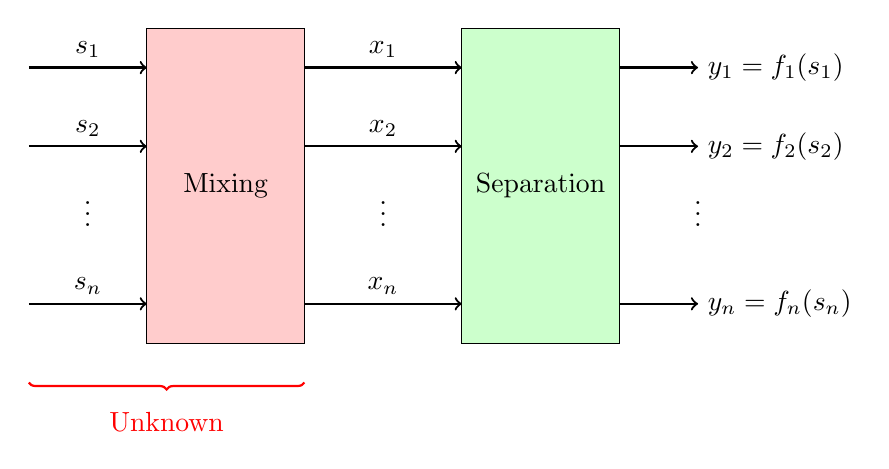
\begin{tikzpicture}

\onslide<1->{
\filldraw[draw = black, fill = red!20!white] (0,0) rectangle (2,4);
\node (text) at (1,2){Mixing};

\foreach \x in {0.5, 2.5, 3.5}
{
	\draw[->, thick] (-1.5, \x) -- (0, \x);
}

\node (vdotsin) at (-0.75,1.75){$\vdots$};


\node [anchor=south] (vdotsin) at (-0.75,0.5){$s_n$};
\node [anchor=south] (vdotsin) at (-0.75,2.5){$s_2$};
\node [anchor=south] (vdotsin) at (-0.75,3.5){$s_1$};


\foreach \x in {0.5, 2.5, 3.5}
{
	\draw[->, thick] (2, \x) -- (4, \x);
}

\node (vdotsin) at (3,1.75){$\vdots$};

\node [anchor=south] (vdotsin) at (3, 0.5){$x_n$};
\node [anchor=south] (vdotsin) at (3, 2.5){$x_2$};
\node [anchor=south] (vdotsin) at (3, 3.5){$x_1$};
}
\onslide<2->{
\filldraw[draw = black, fill = green!20!white] (4,0) rectangle (6,4);
\node (text) at (5,2){Separation};

\foreach \x in {0.5, 2.5, 3.5}
{
	\draw[->, thick] (6, \x) -- (7, \x);
}
\node (vdotsin) at (7,1.75){$\vdots$};

\node [anchor=west] (vdotsin) at (7, 0.5){$y_n = f_n(s_n)$};
\node [anchor=west] (vdotsin) at (7, 2.5){$y_2 = f_2(s_2)$};
\node [anchor=west] (vdotsin) at (7, 3.5){$y_1 = f_1(s_1)$};
}
\onslide <2->{
\draw [
red, thick,
decoration={
	brace,
	mirror,
	raise=0.5cm
},
decorate
] (-1.5, 0) -- (2, 0);

\node [red, anchor=north] at (0.25, -0.75){Unknown};

}
\end{tikzpicture}
\end{figure}
\end{frame}



\section{Linear and Non-Linear BSS}
\begin{frame}
\frametitle{Linear and Non-Linear BSS}
\begin{alertblock}{Darmois-Skitovic Theorem \small{[Darmois-Skitovich ∼1950]}}
In the linear setting, the model is identifiable if the sources are \textbf{non-Gaussian} random variables.
\end{alertblock}
\pause
\begin{exampleblock}{Non-Linear Mixtures}
Non-linear mixtures are harder!
\small{
\begin{equation*}
\begin{cases}

S_1 = \mathrm{Rayleigh}(\sigma)\\
S_2 = \mathrm{Uniform} [0, 2\pi]
\end{cases}
\implies
X_1 = S_1 \cos (S_2) \perp \!\!\! \perp X_2 =  S_1 \sin (S_2)
\end{equation*}
}
\end{exampleblock}
\end{frame}
\normalsize

\section{Using Time Structure of the Data}
\begin{frame}
\frametitle{Using Time Structure of the Data}
\begin{block}{Time relations can help! \small{[Hosseini et al., 2003]}}
The output \textbf{Stochastic Processes} are not independent.
	\begin{align*}
	R_{x_1x_2}(t, t+1) &= \mathbb{E}\big[{x_1(t+1)x_2(t)}\big]\\
	&= \mathbb{E}\Big[s_1(t+1)s_1(t)\Big]
	\mathbb{E}\Big[\cos\big(s_2(t+1)\big)\sin\big(s_2(t)\big)\Big]
	\end{align*}
\end{block}  
\end{frame}

\section{New Separability Results}
\begin{frame}
\frametitle{New Separability Results}
	\begin{alertblock}{Permutation Contrastive Separation [\footnotesize{Hyvarinen et al., 2017}]}
The mixture
		$\textbf{x}(t) = \textbf{f}\big(\textbf{s}(t)\big)$ is separable if:
		\begin{itemize}
			\item
			$\textbf{f}$ is invertible and smooth!
			\item
			$s_i(t)$:  \textbf{stationary},  \textbf{ergodic} and  \textbf{ \textit{uniformly dependent}}.
			\item
			$s_i(t)$ are not \textbf{ \textit{quasi-Newton}}.		
		\end{itemize}
	\end{alertblock}
\pause
	\begin{block}{Time Contrastive Learning \footnotesize[{Hyvarinen et al., 2016}]}
The mixture
$\textbf{x}(t) = \textbf{f}\big(\textbf{s}(t)\big)$ is separable if:
\begin{itemize}
\item
$
	\log p_\tau(s_i)=    \lambda_{i}(\tau) q(s_i) - \log Z( \lambda_{i}(\tau))
	\label{eq:p_tau_simple}
$
\item
$[\mathbf{L}]_{\tau, i} = 
	\lambda_{i, 1}(\tau) - \lambda_{i, 1}(1) \
	$
	has full column rank.
\end{itemize}
%	$$\Rightarrow \exists \mathbf{A} \in \mathbb{R}^{n\times n}
%	\;\;\; \exists\mathbf{d} \in \mathbb{R}^n
%	\;\;\;\;\;
%	q(\mathbf{s}_t) = \mathbf{Af^{-1}}(\mathbf{x}_t) + \mathbf{d}$$
\end{block}
\end{frame}

\section{This Project}
\begin{frame}
\frametitle{This Project}

\begin{block}{Generalized TCL}
Generalize TCL for $$
	\log p_\tau(s_i)=  q_{i,0}(s_i) + \sum_{v=1}^V \lambda_{i,v}(\tau) q_{i,v}(s_i) - \log Z( \lambda_{i,1}(\tau),\ldots,\lambda_{i,v}(\tau))$$
\end{block}

\pause
\begin{alertblock}{Sparse Signals}
	If the signal is sparse in time, BSS is easy! What if it is sparse in some other domain?
\end{alertblock}

\end{frame}


\begin{frame}


\begin{exampleblock}{Separation Algorithms}
	\vspace{0.2cm}
	Generalizing Information Minimization Algorithms for Non-Linear BSS.  \scriptsize{[Babaie-Zadeh et al., 2005]}
\end{exampleblock}



\pause
	\begin{alertblock}{Final Goal (?)}
		A General Indentifiability Result for Smooth Mixtures. Is Smoothness Enough\\
		 \textbf{Idea}: Nonlinear BSS is linear in an specific high dimensional feature space.
	\end{alertblock}

\end{frame}

\section{Bibliography}
\begin{frame}[t, allowframebreaks]
\frametitle{Selected Papers}
\scriptsize{
\bibliography{bib}
\nocite{shahram,TCL, PCL,comon2010handbook, babaie2005general}
\bibliographystyle{plain}
}
\end{frame}

\framecard{Thank You!}


\end{document}